PMTs are used in the TRITIUM experiment for two main objectives. On the one hand, to determine the amount of incident photons that reach the PMT photocathode and, on the other hand, to measure the energy spectrum of tritium events in the laboratory prototypes.

To determine the amount of photons reaching the photocathode, the PMT should work without gain which is a source of uncertainty. For this, the bias circuit shown in Figure \ref{fig:ElectronicSchemeBasePMTNoGain} was employed. As electrons are not multiplied, the output current of the photosensor is very small (currents in the nanoampere range). This output current was readout system by the Keithley 6487 Picoammeter/Voltage Source \cite{DataSheetKeithley6487}. 

The energy of the events was measured with the voltage divider shown in Figure \ref{fig:VoltageDividerCircuit}. The number of PMTs used simultaneously was one, two or four, depending on the setup. A scheme of the electronics employed in each case, based on various NIM modules\footnote{The Nuclear Instrumentation Module (NIM) is a standard specification convention for electrical and mechanical parameters defined in electronic modules used in experimental nuclear and particle physics.}, is shown in Figures \ref{subfig:ElectronicConfiguraiton1PMT}, \ref{subfig:ElectronicConfiguraiton2PMT} and \ref{subfig:ElectronicConfiguraiton4PMT}, respectively.

\begin{figure}
\centering
    \begin{subfigure}[b]{1.0\textwidth}
    \centering
    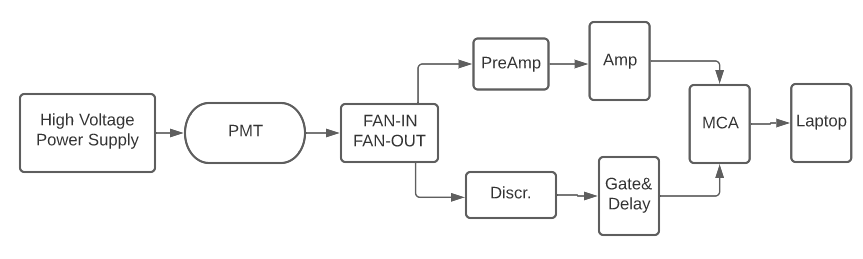
\includegraphics[width=\textwidth]{3DesignPrinciples/32Tritium_detector/Electronical_Scheme_1_PMT.png}  
    \caption{\label{subfig:ElectronicConfiguraiton1PMT}}
    \end{subfigure}
    \hfill
    \begin{subfigure}[b]{1.0\textwidth}
    \centering
    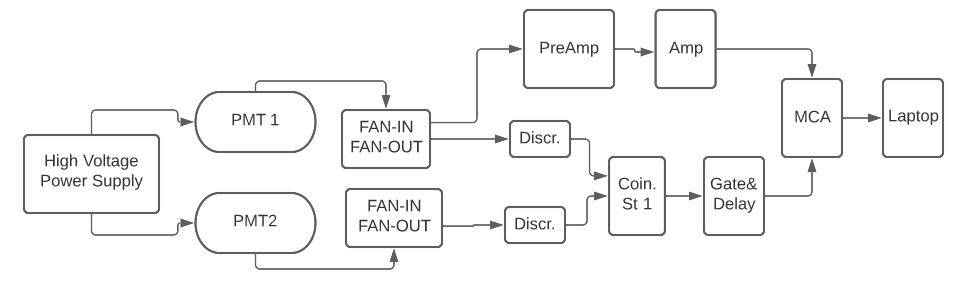
\includegraphics[width=\textwidth]{3DesignPrinciples/32Tritium_detector/Electronical_Scheme_2_PMTs.png}  
    \caption{\label{subfig:ElectronicConfiguraiton2PMT}}
    \end{subfigure}
    \hfill
    \begin{subfigure}[b]{1.0\textwidth}
    \centering
    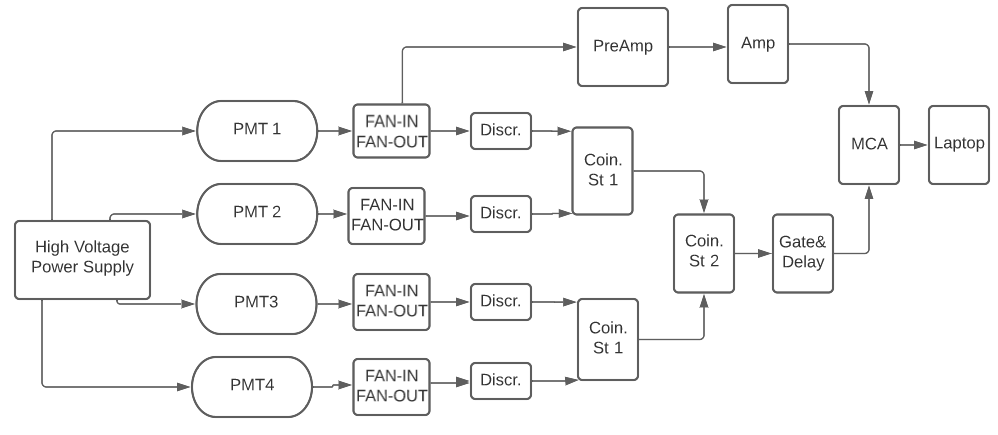
\includegraphics[width=\textwidth]{3DesignPrinciples/32Tritium_detector/Electronical_Scheme_4_PMTs.png}  
    \caption{\label{subfig:ElectronicConfiguraiton4PMT}}
    \end{subfigure}
 \caption{Schemes of the different electronics for measuring with PMTs. a) Employed with only one PMT. b) Employed with two PMTs in time coincidence. c) Employed with four PMTs in time coincidence.}
 \label{fig:ElectronicConfiguraitonsPMT}
\end{figure}

The PMTs were powered by a TC 952 High Voltage Supply from Tennelec \cite{DataSheetHVSupplyTennelec} and a HV Power Supply N 1130-4 from Wenzel Elektronik company \cite{DataSheetHVSupplyWenzel}, each with 4 channels. As can be seen in the figures, the PMT output signals were splitted by an analogic FAN IN-OUT to feed the amplification line that gives the energy spectrum and the time coincidence line. The one employed was the Quad linear FAN IN-OUT MODEL 740 from Philips Scintific \cite{DataSheetFANINOUT}, which has four channels. One output signal was used for the amplification line and the second for the time coincidence electronics.

\begin{enumerate}

\item{} The amplification line is the same for the three configurations and provides the energy information. It consists of two steps:

%We have to take into accout that we have only used the signal from one PMT for the amplification part. We could have added a stage where we add the four PMT output signals and it would probably improve our results, but since our ultimate goal is to work with SiPM, we have not delved into that.

%The electronic path we have followed to achieve this amplification is:

\begin{enumerate}

\item{} The PMT signal is integrated by a preamplifier, which gives an output signal with a heigth proportional to the charge of the input pulse. This signal has a long tail\footnote{The length of the tail is, $\tau=RC$, where R is the input resistance and C is the capacitance used. It is the typical output signal in RC circuits.} produced by the preamplifier capacitance. The preamplifier used was "MODEL 9326 FAST PREAMP" from ORTEC \cite{DataSheetPreAmp}.

\item{} The output signal from the preamplifier is lead to the amplifier which gives a Gaussian shaped output signal. The amplifier modules were 575A and 671 from ORTEC \cite{DataSheet575Amp, DataSheet671Amp}. An example of the 575A module output signal is shown in Figure \ref{fig:InputSignalsMCA}, green color.

\end{enumerate}

\item{} The time coincidence line contains the time information and gives the coincidence gate for the PMT signals. This line consists of the following branches,

\begin{enumerate}

\item{} The PMT output signal is introduced into a discriminator module that gives a logic signal of $-1.2~\volt$ height and of $240~\nano\second$ width when a given threshold is exceeded. The discriminators employed are a Octuple Constant-Fraction Discriminator CF8000 module from ORTEC \cite{DataSheetDiscriminator} and 4 channels discriminator model 84 from CAEN \cite{DataSheetDiscriminatorCAEN}.

\item{} Time coincidences are required to ensure that detected events come from the same tritium decay and to remove external light and dark current. The two logic signals given by the discriminator are introduced in a coincidence module which generates an output signal of $-1.4~\volt$ heigh and of $20~\ns$ width when both imputs are in time coincidence. The modules used were Coincidence Unit Model 465 from LeCroy \cite{DataSheetCoincidenceLeCroy} and Coincidence Type N6234 from CERN-NP \cite{DataSheetCoincidenceCERN}.

\item{} Time coincidence of two different detectors (4 PMTs, configuration \ref{subfig:ElectronicConfiguraiton4PMT}) is use to remove background due to hard cosmic rays. The coincidence signal from both detectors are checked for coincidence.

In Figure \ref{fig:DifferentCoincidences}, time coincidences of two detectors (4 PMTs) are shown. The four logical signals are displayed, two of them from each detector. The possible cases are:

\begin{enumerate}
\item{} Only one PMT (channel two) detected an event as shown in Figure \ref{subfig:signalInOnePMT}. It means that the event is likely not produecd in the scintillator. In this case, no output signal is generated.

\item{} Two PMT signals are generated but the other detector gives no signal as shown in Figures \ref{subfig:signalInTwoPMTOneDetector} and \ref{subfig:signalInTwoPMTOtherDetector} . This event is discarded.

\item{} The four signals are generated as shown in Figure \ref{subfig:signalInAllPMTsBothDetector}  and, consequently, the output signal is generated and the event is recorded.

\begin{figure}
\centering
    \begin{subfigure}[b]{0.45\textwidth}
    \centering
    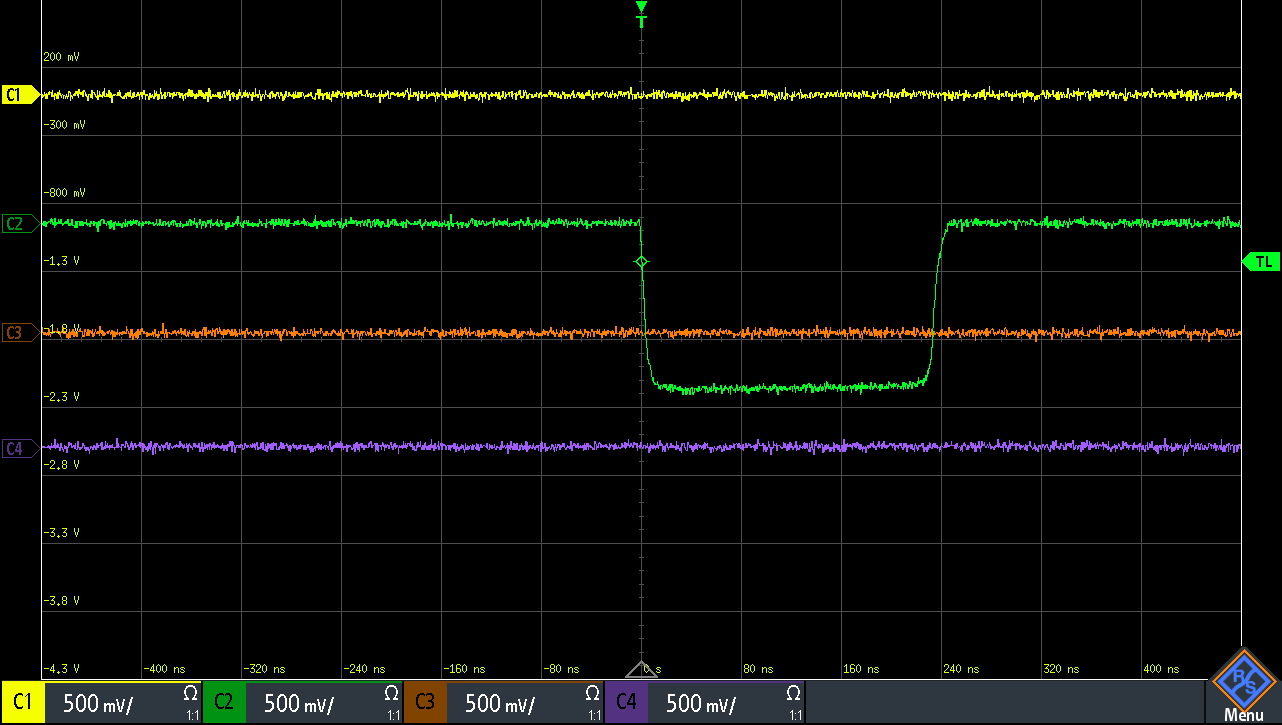
\includegraphics[width=\textwidth]{3DesignPrinciples/32Tritium_detector/1_coincidences.png}  
    \caption{\label{subfig:signalInOnePMT}}
    \end{subfigure}
    \hfill
    \begin{subfigure}[b]{0.45\textwidth}
    \centering
    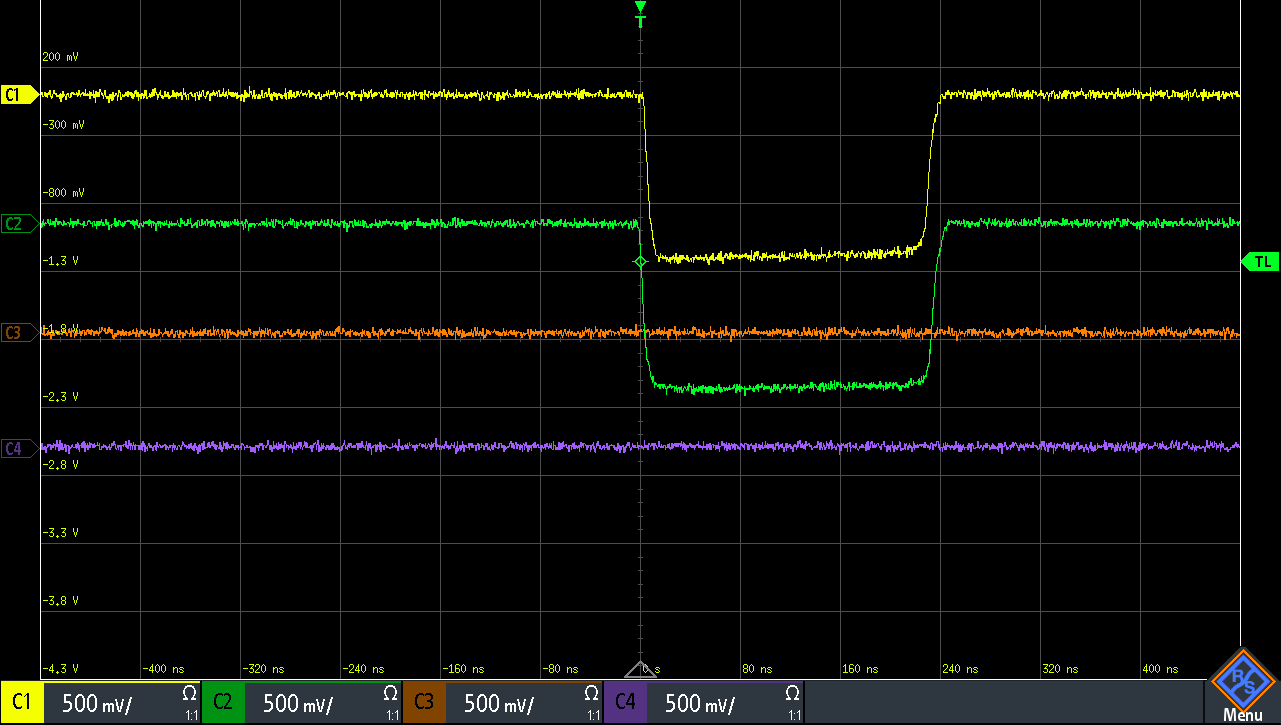
\includegraphics[width=\textwidth]{3DesignPrinciples/32Tritium_detector/2_coincidences_1.png}  
    \caption{\label{subfig:signalInTwoPMTOneDetector}}
    \end{subfigure}
    \hfill
    \begin{subfigure}[b]{0.45\textwidth}
    \centering
    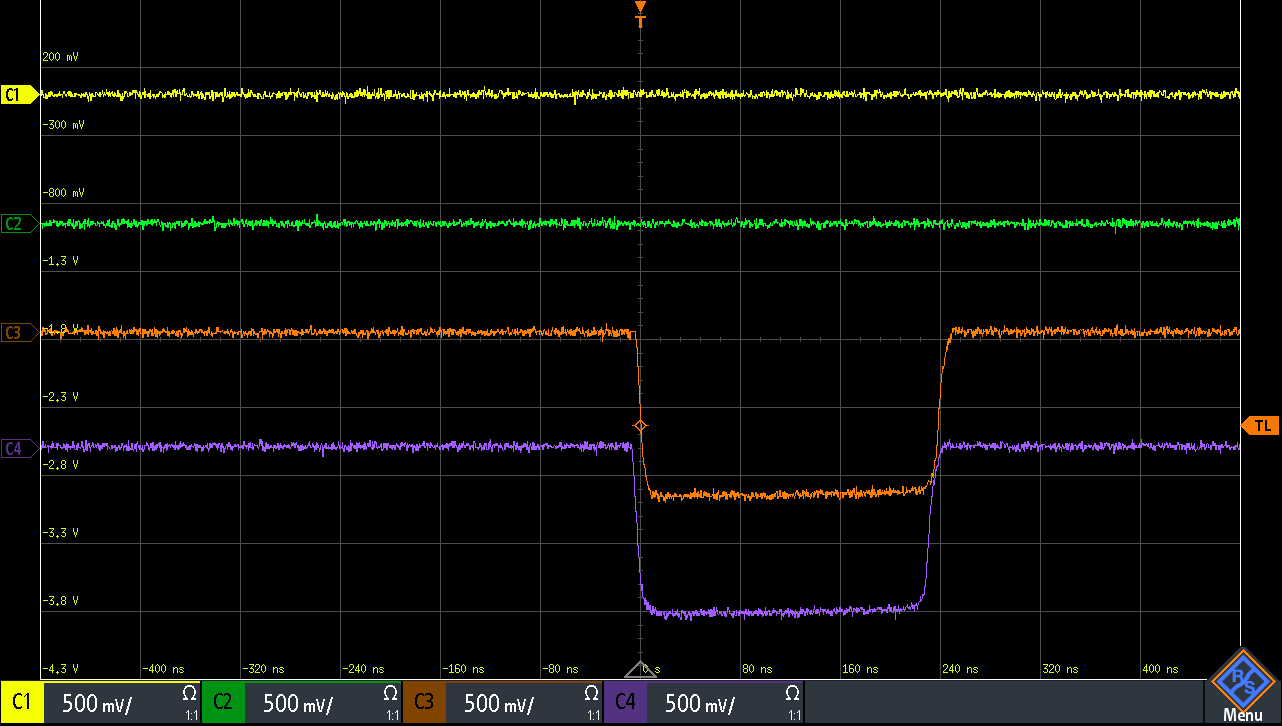
\includegraphics[width=\textwidth]{3DesignPrinciples/32Tritium_detector/2_coincidences_2.png}  
    \caption{\label{subfig:signalInTwoPMTOtherDetector}}
    \end{subfigure}
    \hfill
    \begin{subfigure}[b]{0.45\textwidth}
    \centering
    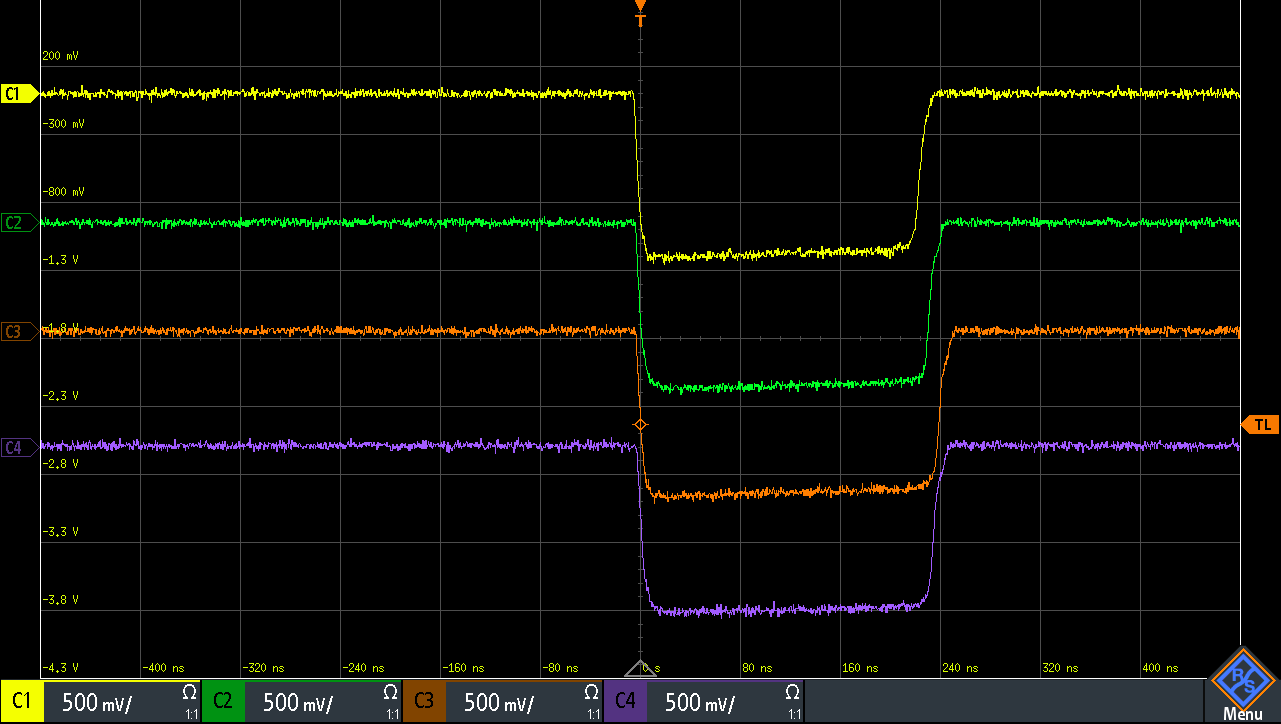
\includegraphics[width=\textwidth]{3DesignPrinciples/32Tritium_detector/4_coincidences.png}  
    \caption{\label{subfig:signalInAllPMTsBothDetector}}
    \end{subfigure}
 \caption{Different possibilities when time coincidences with two detectors are done. Two signals (yellow and green) come from two PMTs reading the first detector and the other two signals (color orange and violet respectively) come from PMTs reading the second detector. a) Event detected in only one PMT detector. b) Event detected in two PMTs, first detector. c) Event detected in two PMTs, second detector. d) Event detected in both detectors.}
 \label{fig:DifferentCoincidences}
\end{figure}

\end{enumerate}

\item{} The logical output signal, is introduced in a Gate and Delay Generator, model 416A from ORTEC \cite{DataSheetGateAndDelay}, which gives a positive logical signal $8~\volt$ height and $2~\mu\second$ width. This module delays the time windows until they overlap with the energy signal as shown in Figure \ref{fig:InputSignalsMCA}.

\end{enumerate}

\end{enumerate}

The final output of the electronics are a logical and analogical signals, shown in Figure \ref{fig:InputSignalsMCA}, which are recorded by the MCA 8000D, Pocket MCA from AMPTEK \cite{DataSheetMCA}. The analogical signal gives the information about the energy of the event and is saved for later analysis whenever it is within the logical signal windows.

\begin{figure}[htbp]
\centering
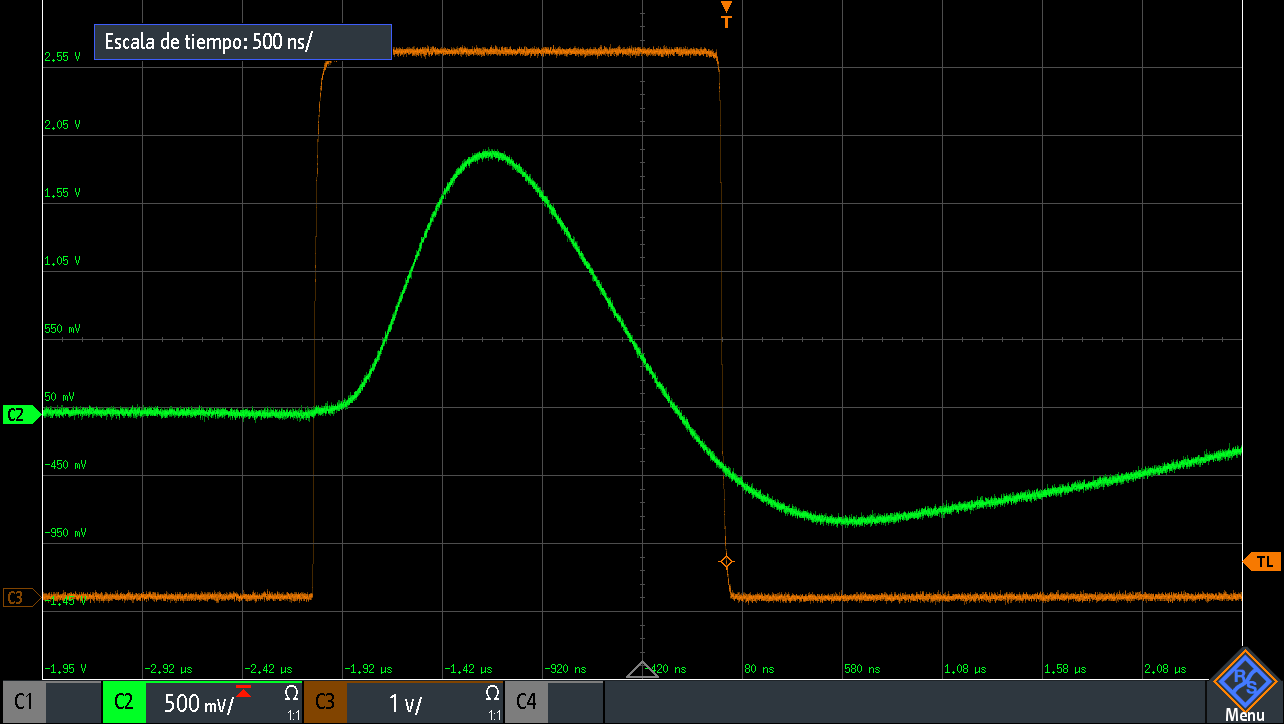
\includegraphics[scale=0.3]{3DesignPrinciples/32Tritium_detector/Input_MCA.png}
\caption{Signal amplified and logical gate (input signals of MCA).\label{fig:InputSignalsMCA}}
\end{figure}